% LaTeX Document Template
% Made by Adnan Berberovic
% Contact by:
%	E-mail: adnbe196@student.liu.se
%	Phone: 070-49 19 607

\documentclass[11pt]{article}
\usepackage[margin=3cm]{geometry}
\usepackage[swedish]{babel}
\usepackage[utf8]{inputenc}
\usepackage[T1]{fontenc}
\usepackage{fancyhdr}
\usepackage{ragged2e}
\usepackage{titling} % Make custom titles.
\usepackage{graphicx} % Allow graphics.
\usepackage{pbox} % Used for margins in tables.
\usepackage{tabularx} % Used for tables.
\usepackage{longtable} % Used for tables.
\usepackage{tabu} % Used for tables.
\usepackage{url} % Allow urls.
\usepackage{amsmath} % Allow math \begin{equation}, end
\usepackage[backend=bibtex,style=ieee]{biblatex} % Bibliography package.
\usepackage{csquotes} % Spawns an error if not included. Not sure why.
\usepackage[hidelinks]{hyperref} % To include urls, hyper links and clickable references
\usepackage[nottoc]{tocbibind} % To include bibliography in ToC

\pagestyle{fancy}
\date{} % Sets date to blank.

\pagenumbering{roman} % Set roman page numbering before the actual document begins.
\chead{TYPE OR TITLE OF REPORT} % Replace argument with the type or title of your report.
\rhead{DATE} % Set date here.
\lhead{} % Put anything here.
\lfoot{COURSE\\INSTITUTION} % Replace COURSE with the course code, INSTITUTION with respective institution.
\rfoot{AUTHOR} % Replace AUTHOR with your name. Add more text if you deem it necessary.

\graphicspath{ {images/} } % Set graphics path if images are to be used in document

\addbibresource{refs.bib} % Import reference bibliography

% Use this command, and make more if you need, to keep some kind of numbering order,
% without the need to replace numbers if something in your list needs to be removed/added.
% To make more, just copy and paste the following 6 lines and replace "cter" with the counter
% name, ccounter with the command name you wish to use. (Remember to replace \thecter with
% \the"newname").
\newcounter{cter}
\setcounter{cter}{1}
\newcommand{\ccounter}{
	\thecter.
	\stepcounter{cter}
}

\begin{document}
	\begin{titlepage}
		\begin{center}
			
			{\Large\bfseries NAME OF DOCUMENT} \\ % Replace "NAME OF DOCUMENT" with... you know.
			
			\vspace{2\baselineskip}
			
			AUTHOR, \textit{autho123} \\ % Replace AUTHOR with your name and autho123 with your ID.
			
			\vspace{2\baselineskip}
			
			YYYY-MM-DD	% Replace with date.
			
		\end{center}
	\end{titlepage}
	
	\setcounter{secnumdepth}{0} % Prevent numbering of the following sections.
	\section*{Abstract}
	
	CONTENT OF ABSTRACT 
	\pagebreak
	
	\setcounter{secnumdepth}{2} % Resume numbering of the following sections.
	
	\tableofcontents	% Make a ToC.
	
	\pagebreak
	
	
	\pagenumbering{arabic}	% Start page numbering with arabic numbers, for the rest of the document.
	
	\section{Section} 	% Example section, 
	
	CONTENTS OF SECTION
	
	\begin{table}[h]
		\begin{tabular}{|l|l|} \hline
			
			Example&
			Table \\ \hline
			
			1&
			2 \\ \hline
			
		\end{tabular}
	\end{table}
	% The block above is a table block. Change the |l|l| to how many columns you desire. l could be something else.
	% Check LaTeX reference for how to manage a table.
	
		\begin{center}	%Example figure, center and import from the images directory.
			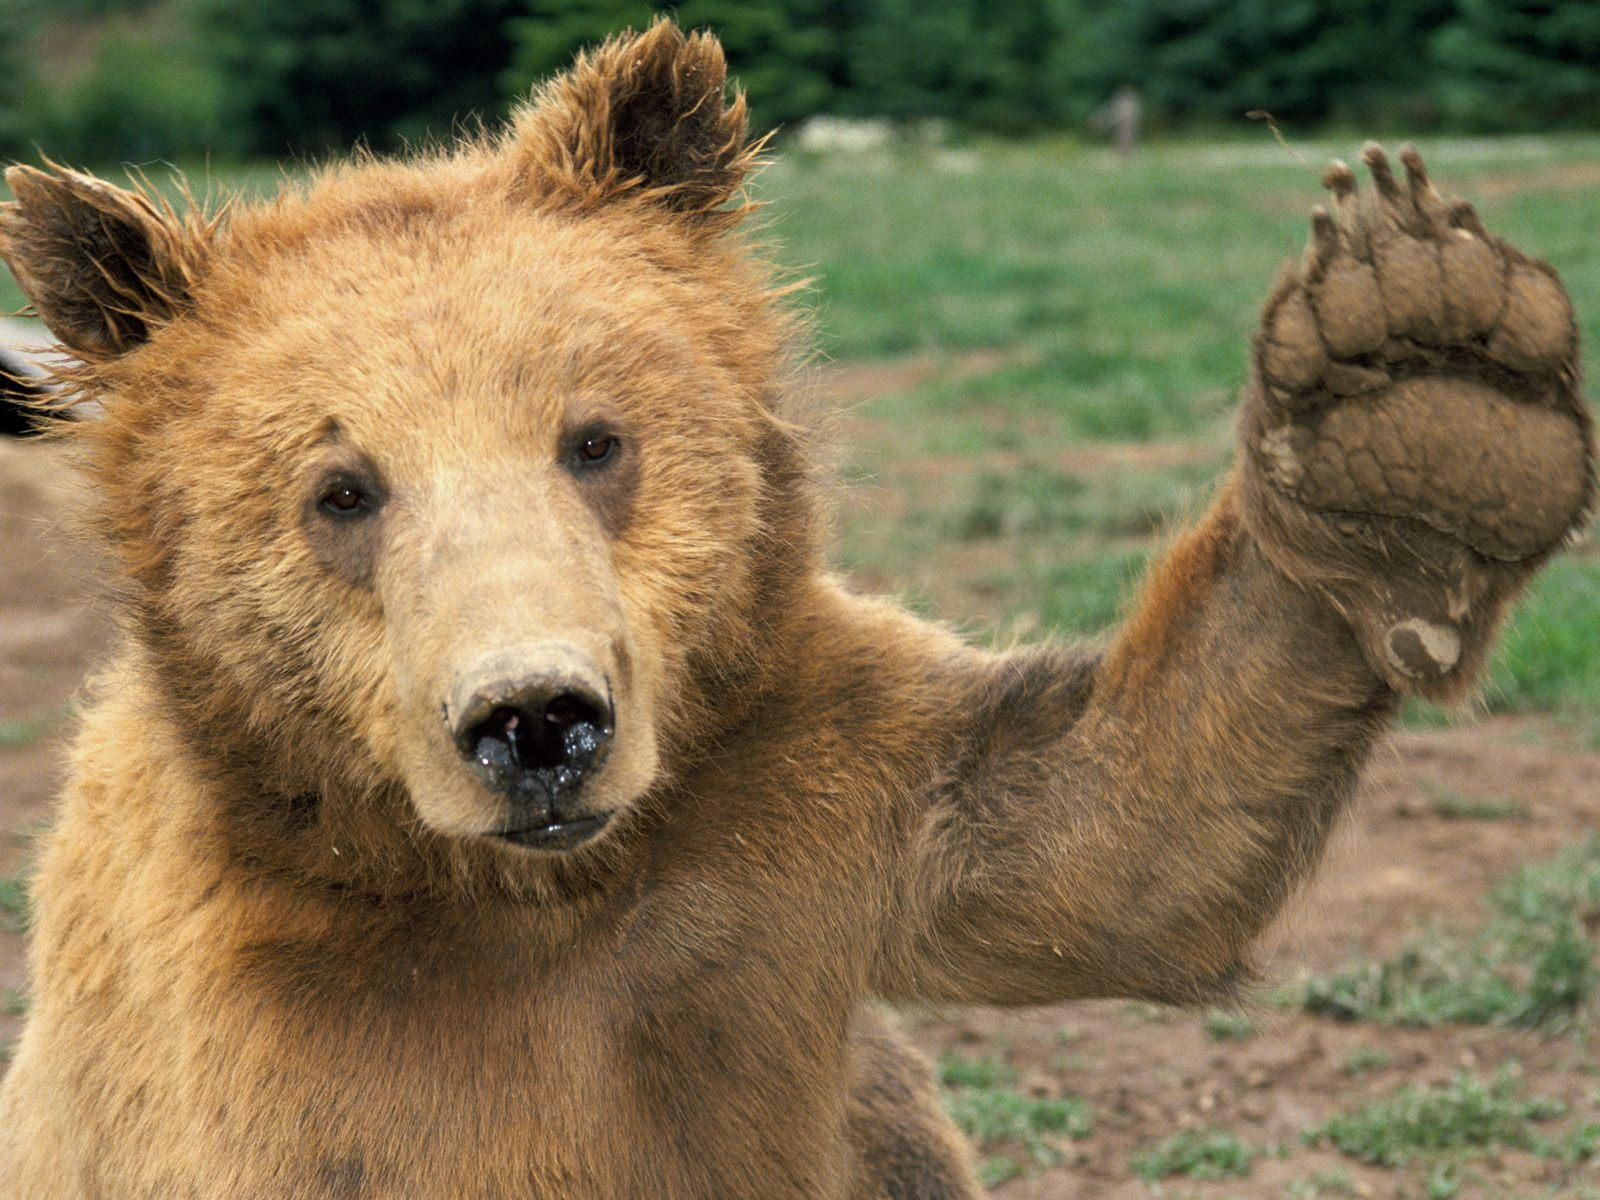
\includegraphics[scale=0.1]{example_pic}\\ % Scale if needed, replace example_pic with name of picture.
			\textit{Figure\ccounter Short description of this figure.}
		\end{center}
		
	\subsection{Subsection}
	
	CONTENTS OF SUBSECTION
	
	\begin{equation}
		ab = ba	% Equation example. Use LaTeX reference page for how to format equations.
	\end{equation}
	
	\begin{itemize}
		\item First item % Item list example.
	\end{itemize}
	
	Citation from reference \autocite{glad-06}
		
	\pagebreak
		
	\setcounter{secnumdepth}{0} % Prevent page numbering yet again. 
	\addcontentsline{toc}{section}{Referenser} % Add reference to ToC. Might have to compile TWICE.
	
	\printbibliography % Prints bibliography. Check refs.bib file in same directory and make sure you have all
	% references at hand when autociting them.
	
	\pagebreak
	
	\section{Appendix}
	\subsection{Appendix A} % Appendix if needed. Comment or delete this section if not useful for your document.
	
	Appendix A contents.
\end{document}
	
	